\chapter{Vybraná témata v~pojetí Karla Makoně}
\label{kap:temata}

Z~toho mála, co o Karlu Makoňovi bylo napsáno a publikováno, se většina týká
nevšedních epizod jeho života, popřípadě zhodnocení jeho díla či nástin některé
jednotlivosti jeho obsáhlé nauky. Moje disertační práce z~tohoto vybočuje tím,
že se snaží aspoň nástínit seznam témat, kterým se Makoňovo dílo věnuje. Toto
úsilí bych rád rozvedl v~této kapitole a rád bych, aby pokus o zmapování
hlavních prvků Makoňova poselství byl hlavním přínosem této diplomové práce.

Vzhledem k~samotné kvantitě Makoňova díla je tento můj záměr téměř bláhový. Sám
jsem přečetl jen šest Makoňových knih a poslechl asi třetinu jeho
dostupných nahrávek. Vzhledem k~tomu, že přístupnost Makoňových nahrávek je
z~velké části mým dílem, na kterém jsem strávil více než dekádu, a k~tomu, že
prakticky všechny dosavadní zmínky o Makoňově díle se soustředí na jeho knihy,
dává mi smysl na moje předchozí úsilí navázat a soustředit se na nahrávky.

Záměr zmapovat množinu hlavních poselství v~Makoňově díle vychází krom jiného
také z~toho, že po poslechnutí většího množství nahrávek docházím k~pozorování,
že navzdory velké rozmanitosti otázek, které Makoň zodpovídá, se vývody
v~odpovědích s~obměnami opakují. Do jaké míry se opakují, jak moc zůstávají
výpovědi napříč vývojem Makoňovy nauky obsahově totožné, a kolik vlastně
takových opakujících se sdělení je, jsou hlavní otázky, které si pokládám.

Určitá sdělení se
neustále vracejí a ačkoliv je pokaždé trochu jiné, ve stěžejních bodech zůstává
stále totéž. Mohu uvést několik příkladů takových sdělení, se kterými se
opakovaně u Karla Makoně setkávám:

\begin{enumerate}
  \item{
      Cesta k Bohu se dělí na fáze. Podle toho, kde se nacházím, platí pro mě
      jiné zákonitosti.  Mezi fázemi jsou ostré předěly.
  }
  \item{
      Pro spojení s Bohem je zapotřebí vrcholné aktivity i absolutní pasivity.
  }
  \item{
      Modlitba nesmí být mechanická, musí být autentická.
      Prosebná modlitba má smysl jako prostředek na cestě.
      ,,Modlete se neustále`` dokazuje, že nejlepší modlitba není slovní, ba ani neznamená myslet na Boha.
  }
  \item{
    Ježíš bojoval proti osudovosti.
    Nejsme v rukou osudu, ale jsme vedeni událostmi ke spojení s Bohem.
  }
  \item{
    Satan je naše \textit{já}.
    \textit{Já} je potřeba rozvinout a přemoci zapřažením do úkolu.
    Světci byli pronásledováni Satanem, protože nechávali svoje \textit{já} zahálet.
  }
  \item{
    Ctnosti nestačí, naopak člověku brání v postupu, když se s nimi ztotožňuje.
    Ctnostný život nevede do nebe, pokud se ctnosti neopustí.
    Člověk musí být nic.
  }
  \item{
    Ráj je stav, ze kterého jsme padli, a není našim cílem.
    Je zastávkou na cestě a oklikou.
    Ráj zažívají zvířata ve spánku.
    Pohlavní pud nebo touha po alkoholu jsou projevem touhy po ráji.
    Nebe je stav, ze kterého nelze vypadnout.
    Ve stavu nebe je člověk více činný než v běžném životě.
  }
  \item{
    Katolická tradice je nedoceněná, mělo by se na ni navázat, ale musí se korigovat.
  }
  \item{
    Do spojení s Věčností lze vstoupit jen celobytostným sebeodevzdáním.
  }
  \item{
    Boží milost je zákonitá, není nevyzpytatelná.
    Podmínky jsou plné rozvinutí hlavní složky života a její bezpodmínečné odevzdání.
  }
  \item{
    Stvoření neproběhlo, ale probíhá.
    Genesis hovoří o vzniku člověka po duchovní i tělesné stránce.
  }
  \item{
    Každý prostředek na cestě má omezenou platnost, včetně víry.
    Cíl musí být vždy nejvyšší, a to vědomé spojení s Bohem.
    Království Boží je stav, kdy v člověku kraluje Bůh.
  }
  \item{
    Krize je volání Boží.
  }
  \item{
    Apoštolové symbolizují lidské vlastnosti.
  }
  \item{
    Křesťanství překonává model reinkarnace tím, že umožňuje vyvázání ze samsáry během jediného vtělení.
    Nepřevtěluje se člověk z těla do těla, ale člověk navazuje a odhazuje karmické balíky.
    Tak lze být převtělením mnoha lidí najednou a jeden člověk se vtěluje do mnoha jiných.
    Indové se silou představy převtělují tradičně.
  }
  \item{
    Vlastnictví je největším hříchem.
    Máme spravovat, ne vlastnit.
    Ježíš učil především nevlastnit.
  }
  \item{
    Všechno utrpení je způsobeno nerovnováhou mezi vnitřním a vnějším životem.
  }
  \item{
    Láska je jediným prostředkem, který nelze překonat.
    Cesta lásky je jediná, která může být úspěšná i bez krizí.
    Láska člověka vyvádí z něho samého.
    Symbolem lásky byl apoštol Jan.
    Láska je otázkou vůle.
  }
  \item{
    Bible je dokonalým, podrobným symbolickým plánem na cestu k Bohu pro každého člověka.
    Ježíšův život je obecným vzorcem (a² + b²) a naše životy jsou aplikací vzorce.
  }
  \item{
    Panna Maria symbolizuje nesmrtelnou duši.
    Maria jediná člověka nikdy neopouští (byla i pod křížem).
  }
  \item{
    Smrt na kříži symbolizuje mystickou smrt, která musí proběhnout před smrtí fyzickou a je poslední podmínkou vstupu do věčnosti.
  }
  \item{
    Smrt je svlečením hmotného těla a oblečením astrálního.
    Mrtví žijí na úrovni druhé čakry, tamtéž jako my, když sníme.
  }
  \item{
    Krom verbálního existuje i obsahové sdělování.
    Probíhá \textit{en bloc} a napříč jazyky.
    Podmínkou je zastavení povídavé mysli při zachování vědomí.
  }
  \item{
    Extáze je překonaným fenoménem.
    Budoucnost patří cestě bez extází.
    Extáze je nejvyšší stav, kam lze dojít vlastní silou.
  }
  \item{
    Míra sebezáporu (později odosobnění) je měrou duchovního pokroku.
  }
\end{enumerate}

\section{Opakující se výroky}

Dojem o konzistentně se opakujících poselstvích vyvolává otázku, do jaké míry se
témata skutečně opakují a jak se jejich pojetí vyvíjí v~čase. U několika témat
se pokusím tuto otázku zodpovědět.

\subsection{Metodologie}

Vycházím z~kompletně přepsaných zvukových záznamů Makoňových hovorů, kde zčásti
se jedná o přepisy manuální prakticky bez chyb a zčásti automatické s~mírou
chybovosti úměrné akustické kvalitě záznamu, běžně se však pohybující kolem 90\%
správně přepsaných slov. Nutno také podotknout, že i chybně přepsaná slova mají
mnohdy správně určený kmen a pro účely vyhledávání je tedy můžeme považovat za
správně přepsané. Krom toho využívám manuálně vytvořený tematický index
pokrývající v~dubnu 2022 všechny písmenem označené kotouče a kazety označené
ročníkem do osmdesátého pátého, celkem 312 z~1138. V~tematickém indexu je jeden
záznam ke každému úseku s~konzistentním tématem.

Postupuji v~následujících krocích:
\begin{itemize}
\item{
Projdu záznamy tematického indexu a ke každému přiřadím jedno či více
obecnějších témat, do kterých záznam spadá.
}
\item{
Témata s~více než pěti přiřazenými záznamy procházím a pro každé provedu
následovné:
\begin{itemize}
\item{
Určím klíčová slova pro fulltextové vyhledávání, která předpokládám, že povedou
k~úsekům, kde se dané téma pojednává.
}
\item{
Klíčová slova vyhledám v~celém přepisu a setřídím si nahrávky podle počtu
výskytů.
}
\item{
Projdu nahrávky s~velkým počtem výskytů tak, aby pokryly maximální časové
období, preferuji rozestup kolem dvou až tří let mezi dobou pořízení.
}
\item{
Z~každé vyberu krátký úsek (jednu či několik vět), který vyjadřuje mluvčího
postoj k~tématu, je-li to možné.
}
\item{
Nenacházím-li takové úseky, uchyluji se k~nahrávkám s~menším počtem výskytů, a
pokud ani tam nenacházím, ponechám mezi citacemi větší odstup.
}
\item{
Na vybraných úsecích pak vyhodnocuji, v~čem se liší a co mají naopak
společného.
}
\end{itemize}
}
\end{itemize}

Tímto postupem se snažím vyvážit časově efektivní využití dostupných materiálů a
přitom omezit zbytečnou subjektivitu. Subjektivita zde vstupuje i tak v~několika
bodech. Samotný tematický index byl tvořen ručně, takže sám o sobě zahrnuje
subjektivní interpretaci. Přiřazování záznamů do obecnějších témat je dalším
subjektivním krokem. Výběr klíčových slov pro vyhledávání je také potenciální
branou subjektivity. Naposledy výběr charakteristických úseků je krokem
s~největší měrou subjektivního zásahu. Aby se subjektivita redukovala, musel by
se postup opakovat několika různými badateli, což je ovšem vysoko nad rámec
možností této diplomové práce. Subjektivitu v~postupu tedy identifikuji a
přijímám jako součást práce, snažím se ji však izolovat a minimalizovat.

Některé manuální kroky by bylo možné nahradit automatickými postupy počítačového
zpracování přirozeného jazyka, ovšem za cenu neúměrného zvýšení náročnosti
provedení.

\subsection{Téma trpnosti}

Trpnost čili pasivitu vykládá Makoň jako jeden z~nejdůležitějších prvků, které
chybějí na cestě jeho posluchačů do vědomého spojení s~Bohem. Ze základního
předpokladu, že člověk má za cíl dojít do Království Božího, mu vyplývá trpnost
jako princip, který může chybět v~dosahování jiných cílů, a jeho zapojení tedy
není samozřejmé, pročež ho vyzdvihuje.

Makoň vychází ze svého stavu, který nastal v~koncentračním táboře, při němž,
budu-li ho parafrázovat, pekročil hranice vesmíru a plně si uvědomoval svoji
nesmrtelnou podstatu. Chtě svým posluchačům dopomoci k~témuž, stojí před
úkolem připravit jiné lidi, aby také překročili hranice vesmíru. Protože každá
činnost směřuje zase do stvořeného, nemohl předat žádný návod založený jen na
činnosti. A protože samotná nečinnost vede k~ustrnutí, nemohl dát návod ani
založený jen na pasivitě. Dává návod postavený na činnosti dovedené na hranice
možností a dokonalém odstupu od takové činnosti a trpném odevzdání se do Boží
vůle. Tento postup je jednak nezbytný a jednak ho přirozeně neprovádíme, což
jsou asi důvody, proč se tomuto tématu tolik věnoval.

Použité vyhledávací vzory: \texttt{aktiv*}, \texttt{trpn*}.

\begin{enumerate}
  \item{
    Nahrávka s~označením \texttt{kotouc-D01-b} od pozice 14:14. Rok pořízení neznámý, ale
    jistě v~sedmdesátých letech.

    Citace: \textit{%
      ,,My totiž tady v tomto životě cokoliv dobýváme, tak vždycky to dobýváme
      nějakou aktivitou, že totiž si to přejeme, jdeme za tím, dosahujeme to,
      případně nedosahujeme. A jakou to činnost? Jak ji máme klasifikovat,
      takovou činnost? To je vlastně pokračování v tvůrčí činnosti Boží. My tady
      rozmnožujeme statky, které jsou nám od Boha dány, a dále prostě pro ně
      žijeme a dále jdeme do stvořeného, do zmnožného. Jde ta cesta z
      jednoduchosti do množství, do stále větší šíře, ano? To je, to je
      tenhleten, ta aktivita. Tímto způsobem když člověk přistupuje i k
      duchovním úkolům, to znamená k tomu, aby se stal nezrozeným, věčným to
      znamená nezrozeným, věčným, nestvořeným, tak když tímto způsobem
      postupuje, tak nikdy se jím nestane, i když se sebepilněji snaží, protože
      mu chybí tahleta zpětná vazba, ta pasivita. On zná jenom ten aktivní
      způsob a ten vlastně jde úplně opačným směrem než ta trpnost mystická,
      která je zapotřebí stejnou měrou jako ta aktivita a kterou jedinou se
      můžete dostat nazpátek.``
    }

    Jedná se o fundamentální výrok o trpnosti, kde Karel Makoň kompaktně uvádí,
    proč ji považuje za důležitou a doplňuje o letmé nastínění principů, které
    ji důležitou činí.
  }
  \item{
    Nahrávka s~označením \texttt{kotouc-I01-d} od pozice 04:20. Rok pořízení rovněž neznámý, ale
    spadající do sedmdesátých let.

    Citace: \textit{%
      ,,Ve skutečnosti každý člověk na všechno hledí aktivně, i na mystickou
      modlitbu, i na modlitbu, která má ho spojit s Bohem a dopadá to potom
      příšerně. Podívejte se na všechny žáky Weinfurtrovy, kdy oni říkali
      nějaká písmenová cvičení, já proti tomu nic nemám, ale mysleli si, že
      tímhletím dobydou Království Boží. Jo, Království Boží násilí trpí,
      násilím je dobýváno, ale ne dobyto. Dobýváno. A oni u toho dobývání
      zůstali, museli zůstat, protože nikdo jim neřekl, že modlitba se musí
      stávat postupně stále více trpnou. Trpnější. Pasivní. A jestliže tento
      požadavek není splněn, tak nemůže vést ke spojení, vědomému spojení s
      Bohem.``
    }

    Příklad školy Karla Weinfurtera z~pohledu Karla Makoně je užit pro
    demonstraci nezbytnosti trpného přístupu. Je zde postulována nezbytnost
    trpnosti pro vstup do Království Božího.
  }
  \item{
      Nahrávka s~označením \texttt{kotouc-77-brezen01-b} od pozice 01:06:02. Rok pořízení 1977.

      Citace: \textit{%
        ,,Trpná stránka, to je stránka koncentrační. Koncentrace není činnost v
        tom běžném slova smyslu, k jaké já vás tady navádím v těchto
        algoritmech. To není ještě koncentrace vůbec. Todleto, k~čemu vás
        já tady navádím, to je nanejvýš meditace, jo? A z ní pocházející čin, čin
        prostý anebo čin láskyplný, ano? Ale koncentrace mystická, ne
        soustředění pouhé, konaná za účelem spojovacím, mající tento cíl, to je
        vyhraněně trpná záležitost. To znamená, já musím se jenom tak dlouho
        koncentrovat, smím lépe řečeno se tak dlouho koncentrovat, dokud
        zůstávám trpný, ale ne civějící.``
      }

      I v~tomto úseku ze sedmdesátých let je důraz kladen na nezbytnost trpnosti
      na cestě ke spojení s~Bohem, tentokrát v~rámci mystické koncentrace.
      Objevuje se zde i pojem civění, který se v~souvislosti s~trpností objevuje
      u Makoně často a který značí trpnost tedy pasivitu nežádoucího druhu.
  }
  \item{
      Nahrávka s~označením \texttt{80-11A} od pozice 19:54. Rok pořízení 1980.

      Citace: \textit{%
        ,,Musím se snažit o to, milovat z celého srdce a tak dále, jak je to tam
        všechno řečeno, ale my jsme si už řekli, že pochopit, kde jsou meze toho
        a kde a jak máme Bohu dát příležitost, aby on nám ukázal svou lásku, to
        že už není, co se dá vyjádřit tím slovem, nýbrž to se dá vyjádřit jedině
        příkladem Ježíšovým. Celým jeho životem.``
      }

      Zde není důraz kladen na potřebnost trpnosti jako takovou, nýbrž na to, že
      najít správné meze mezi činností a trpností není otázkou formulovatelného
      receptu, nýbrž otázkou pochopení příkladu Ježíšova života jako celku.
  }
  \item{
      Nahrávka s~označením \texttt{83-18-K} od pozice 17:51. Rok pořízení 1983.

      Citace: \textit{%
        ,,Už to narození Ježíše Krista vysvětluje značnou míru trpnosti, ale v
        které oblasti, to je mi jasné: Ne všude. Například jakápak je to
        trpnost, když utečou do Egypta? To je velká činnost, ale trpnost je v
        tom, že poslouchali. Vy musíte přesně vědět, že to vedle sebe má
        existovat a že to má své místo, to i ono.``
      }

      Jako v~předchozím úseku je důraz kladen na nalezení mezí aktivity a
      pasivity a navíc na legitimitu obou pólů.
  }
  \item{
      Nahrávka s~označením \texttt{85-25A-10} od pozice 32:53. Rok pořízení 1985.

      Citace: \textit{%
        ,,Láska má dvě stránky: Aktivní a trpnou, ano? To jsem říkal všechny
        čtyři dni. Ne že je to jenom trpná stránka, ale že trpná stránka je
        dovršení oné aktivní stránky lásky. A kdyby to nebylo dovršení aktivní
        stránky, nebylo by co dovršovat a bylo by zbytečné ta negace nebo ta
        trpnost v lásce. By byla bezvýsledná, to by nikam nevedlo.``
      }

      V~tomto úseku pozorujeme ještě silnější odklon on pouhého zdůrazňování
      trpnosti. Důraz je naopak kladen na to, že trpnost, která nenavazuje na
      činnost, nemá význam.
  }
  \item{
      Nahrávka s~označením \texttt{prevzate-kotouc-88-03}. Rok pořízení 1988.
      Uvádím dva úseky.

      První citace, od pozice 11:23: \textit{%
        ,,Vznik i té nejmenší metafyzické zkušenosti je založen na trpnosti.``
      }

      Druhá citace, od pozice 14:08: \textit{%
        ,,Trpnost musí být musí mít protiváhu, že ji dovedete uplatnit, aktivně
        uplatnit. Ježíš Kristus to doved aktivně uplatnit, že byl poddán trpně
        třebas své rodině a tak dále. On, který měl tu obrovskou moudrst za
        sebou, že, a v sobě, který... Takže on to potom už začal nám ukazovat
        jako míchanou trpnost s~aktivitou. A to je správně pojatý život. To má
        být tak namícháno, že když je zapotřebí být aktivní, tak musím být
        aktivní až do dřeně kosti. Když je třeba být trpný, tak musím být trpný
        zase tam.``
      }

      V~první citaci se jedná o postulát nezbytnosti trpnosti, jak jsme viděli u
      raných výroků. Druhá citace opět zdůrazňuje potřebnost obou pólů.
  }
  \item{
      Nahrávka s~označením \texttt{91-11B}. Rok pořízení 1991. Opět uvádím dva
      úseky.

      První citace, od pozice 29:26: \textit{%
        ,,Kdo neumí být trpný, tak není zasvěcencem, a kdo se bojí trpnosti, tak
        neví, že se bojí něčeho, čeho by se neměl bát. To mu umožňuje stát se
        zasvěcencem a být spojen vědomě s~Bohem.``
      }

      Druhá citace, od pozice 38:54: \textit{%
        ,,Ani Ježíš Kristus neudělal první zázrak, a kdyby byl neudělal první
        zázrak za pomoci Panny Marie, tak neudělal ani další zázraky. Začal to
        dělat jenom proto, že ho Panna Maria požádala. Kde pak jsme s~tou
        méněcennosti ženy? Prosím vás, odpovězte mně na to. A protože tomu tak,
        že ona je cennější a v~té trpnosti, která je jí vrozená, je veliká
        přednost a říkáme jí, té přednosti, metafyzická zkušenost, která se bez
        trpnosti, bez stavu trpnosti neobejde, tak my mužové musíme také tuto
        trpnost zvládnout. My ji musíme umět navodit, stejně jako ji umí snáze
        navodit žena.``
      }

      Stejně jako u předchozí nahrávky první úsek postuluje nezbytnost trpnosti.
      Chybí však důraz na potřebnost činnosti. Místo toho uvádí vztah trpnosti
      s~ženským principem.
  }
\end{enumerate}

Nebyl jsem bohužel s~to vybrat nahrávky, které by byly spolehlivě rozdělené
v~kýžených časových rozestupech před rokem 1980, nicméně odstup v~pořadovém
označení kotoučů napovídá, že snad nebyly pořízeny bezprostředně po sobě.

Z~ukázek jasně plyne, že Karel Makoň napříč celým svým zaznamenaným přednáškovým
působením tvrdí, že trpnost je nezbytným prvkem na cestě ke spojení s~Věčností.
V~některých případech je nezbytnost trpnosti podána v~rámci výroku o nezbytnosti
jak činnosti tak trpnosti. Nabízí se hypotéza, že v~raných osmdesátých letech
kladl Makoň důraz na legitimitu činnosti, ovšem tu bychom museli ověřit na
větším vzorku. S~jistotou však můžeme tvrdit, že o nutnosti trpnosti na duchovní
cestě poučoval Makoň vcelku konzistentně po dobu aspoň dvou dekád.

\subsection{Téma modlitby}

Použitý vyhledávací vzor: \texttt{modlit*}.

Téma modlitby se u Karla Makoně objevuje tak často, že nelze opominout. Pro
ilustraci: Slovní tvary obsahující řetězec \texttt{modli} se vyskytují častěji
(16.396\texttimes) než slova jako \textit{potom} (15.278\texttimes) nebo
  \textit{takže} (14.731\texttimes~z~celkových 7.970.485 slovních tvarů). Aspoň
jedna zmínka je ve třech čtvrtinách všech nahrávek.

Podobně jako považuje Makoň za důležité správně skloubit činnost s~trpností,
staví se Makoň i k~modlitbě ve vztahu k~zevnímu životu nebo též k~činnosti. Jako
se musí vhodně střídat úsilí s~odstoupením od úsilí, tak se musí střídat i
orientace vně, do světa, s~orientací do nitra, k~Bohu.

Modlitbou Karel Makoň nerozumí slova pronášená vůči Bohu, ale každé obrácení
pozornosti k~Bohu, vycházeje vždy z~předpokladu ultimátního cíle ve vědomém
spojení s~Bohem, neboli v~prožití vlastní nesmrtelnosti, tedy vstupu do věčného
života.

Jestliže u tématu trpnosti bylo možné vysledovat na několika málo příkladech
uvedenou metodou vývoj v~postoji, u modlitby je pojetí natolik různorodé, že
nebylo vždy možné vybrat výrok, který by byl vhodnou paralelou ostatních
vybraných výroků.

\begin{enumerate}
  \item{
    Nahrávka s označením \texttt{73-01}.
    Rok pořízení 1973.

    První citace, od pozice 01:21:20: \textit{%
      ,,{},Posvěť se jméno tvé, přijď království tvé.` To je to přání, pro které
      my tuto modlitbu vůbec děláme, a jestliže toto přání není naším přáním,
      nemá smysl je vyslovovat a nemá taky smysl od této modlitby očekávat
      spojovací účinek s~Věčností. Nedostaví se.``
    }

    Zpracování Otčenáše není v~hovoru o modlitbě u Makoně žádnou výjimkou, jak
    uvidíme i v~dalších výrocích. Hlavní důraz zde však je na nutnost upřímnosti
    modlitby. Je zde také patrný předpoklad, že posluchač má za cíl vědomé
    spojení s~Bohem.

    Druhá citace, od pozice 01:19:31: \textit{%
      ,,Jestliže jenom jedna jediná naše činnost celého toho dne obsahovala v~sobě
      větší naléhavost než tahleta modlitba, pak vůbec nemá cenu tu modlitbu
      dělat, protože ona nepředežene, nepředběhne náš běžný život a tedy nám
      nebude světlem do dalšího života.``
    }

    Zde je patrné další vyostření toho, že jediným účelem modlitby je vědomé
    spojení s~Bohem. Nedošlo-li k~němu, byla modlitba zbytečná. Vidíme zde též
    pokus o vysvětlení jevů duchovního života pohybovou alegorií.

    Třetí citace, od pozice 01:20:26: \textit{%
      ,,Nesmí se to samo sebou přeříkávat bezmyšlenkovitě jedna myšlenka za
      druhou, nýbrž musíme hledět zažít v~sobě tu čest, která se nám zde
      prokazuje, že naším otcem je bytost nesmrtelná, nekonečná, nejvýš laskavá,
      s~veškerým poznáním a tak dále.``
    }

    Nepřípustnost mechanického způsobu modlitby je dalším opakujícím se motivem
    v~rámci tohoto tématu.
  }
  \item{
    Nahrávka s označením \texttt{76-03B-Kaly-6}.
    Rok pořízení 1976.

    První citace, od pozice 30:36: \textit{%
      ,,Jakéhokoliv nástroje se chopíte, tak se chápáte jenom nástroje. Toto
      bychom měli si být pořád vědomi, protože jinak zaměňujeme, což se často
      stávalo i dobrým žákům této cesty, zaměňujeme tento nástroj za cíl. Takže
      když nám to třeba samo v~nás opakuje jméno Boží, tak si myslíme, kdo ví,
      co se s námi děje. To je jenom tragická záměna nástroje za cíl. Že my jsme
      v~sobě vypěstovali takový automatismus, že samo pořád se to, jak říkají
      někteří z~nich, se to v~nás modlí. To není správné. Já musím záměrně do
      tohoto způsobu modlitby vstupovat a záměrně z~ní vystupovat, protože ona
      je jenom prostředkem. Cílem je vědomé spojení s~Bohem. Vědomé v~tom smyslu
      zpočátku, aspoň v~tom smyslu, že mi poskytuje jistotu, že jsem nesmrtelná
      bytost ve své vnitřní podstatě. A tato jistota se může projevovat i
      přídavnými stavy, ale ty nejsou rozhodující při tom. Rozhodující je tato
      jistota, na které potom buduju nebo postavím celý svůj život. Byl bych
      nerad, aby zdánlivě tento výrok stál proti Ježíšovu výroku: ,Modlete se
      neustále.` To neznamená, podle mého názoru, že by byl Ježíš jakoukoliv
      formu modlitby povýšil na neustálou životní činnost, nýbrž to je něco
      zcela jiného. Podívejte se, ve skutečnosti Ježíš chtěl, aby každý okamžik
      našeho života byl nám tak posvátný, aby se rovnal modlitbě. Ne se podobal,
      rovnal. Aby totiž vás nic v životě neodvádělo od něho, od Boha, nýbrž aby
      nás všecko k Bohu přivádělo. My totiž modlitbu děláme záměrně k~tomu,
      abychom, jak se říká lidově, rozmlouvali s~Bohem nebo abychom se k~Bohu
      přiblížili. Kdežto ostatní děláme proto, abychom provedli to nebo ono, co
      nemá s~tímto duchovním cílem vůbec nic společného. A toto je základní
      rozpor, který Ježíš Kristus vyjádřil ,sedění na dvou židlích`, i když o
      tom mluvil v~jiném smyslu.``
    }

    Záměna prostředku a cíle je samostatné téma, o kterém Makoň často pojednává
    i mimo kontext modlitby. Upření absolutní hodnoty stavu, kdy se modlitba
    v~člověku odehrává samovolně, je podle mojí zkušenosti dosti ojedinělým
    jevem, který ovšem harmonuje s~Makoňovým konzistentním odrazováním od
    ulpívání na konkrétních projevech dosažené duchovní úrovně a na zážitcích
    sebemystičtějšího charakteru.

    Vědomé spojení s~Bohem coby cíl je zde předložen zcela explicitně.
    Ježíšovy výzvy k~neustálé modlitbě se Makoň také dotýká opakovaně.

    Druhá citace, od pozice 36:18: \textit{%
      ,,Člověk pořád pendluje mezi modlitbou a mezi činností. Jedno staví proti
      druhému. Důležité je, aby buď v~té modlitbě anebo v~té činnosti prorazil
      do věčnosti, obojí může.``
    }

    Další příklad zdůraznění modlitby jako protipólu činnosti.
  }
  \item{
    Nahrávka s označením \texttt{prevzate-kotouc-78-03A}, od pozice 06:39.
    Rok pořízení 1978.

    Citace: \textit{%
      ,,Výtěžky modlitby se mají uplatňovat, praktikovat v~zevním životě a zevní
      život se má praktikovat v modlitbě.``
    }

    Opět vytknutí modlitby a činnosti jako vzájemných komplementů.
  }
  \item{
    Nahrávka s označením \texttt{80-18}, od pozice 43:28.
    Rok pořízení 1980.

    Citace: \textit{%
      ,,[Ježíš] spojoval modlitbu se životem. Jeho život byl modlitba, a jestli\-že
      život náš není modlitbou, tak ještě jsme se nezačali modlit.``
    }

    I zde nacházíme modlitbu ve vztahu s~činností, ovšem od pojmu
    \textit{činnost} přechází Makoň k~pojmu \textit{život}. Výrok je vyostřený
    tím, že se upírá opravdovost modlitbě, pokud s~ní neharmonuje celý vnější
    život.
  }
  \item{
    Nahrávka s označením \texttt{82-18}.
    Rok pořízení 1982.

    První citace, od pozice 38:57: \textit{%
      ,,Tak já myslím, že byste mohli rozumět, jak má vypadat prosebná modlitba.
      Když například se někdo modlí Otčenáš, a to je vzor prosebné modlitby,
      všimněte si, co se tam od člověka chce za oběť. Za oběť vůle především:
      ,Staň se vůle tvá. Buď vůle tvá, jako v~nebi, tak i na zemi.` To je tam
      doslova řečeno. ,Přijď království tvé`. Vždyť to je něco, co si člověk
      nepřeje přeci přirozenou cestou. On si přeje: ,Dej nám chléb vezdejší`,
      to možná ano. A aby nepřišel k úrazu, taky. ,Odpusť nám, jako my
      odpouštíme`, to ano. ,Neuveď nás v~pokušení`, to ano. Ale musí
      předcházet, musí být vůdčí myšlenkou při tom tohleto vzdání se do určité
      míry své vlastní vůle. Jiná manipulace s~vůlí, jak jsem to nazval obecně.
      Tak takhle vypadá prosebná modlitba.``
    }

    Prosebné modlitbě jako podtématu modlitby obecně se Makoň také věnuje
    opakovaně. Z~toho, že zmínku nacházíme až ve vzorku z~roku 1982 nelze
    dovozovat, že by se tématu do té doby nevěnoval. Naopak, zvýšený výskyt
    řetězce \texttt{prosebn} nalézáme v~nahrávkách z~let 1979 až 1982 a pak až
    v~roce 1986. Nejvyšší počet výskytů z~celého korpusu je právě v~nahrávce
    \texttt{82-18}.

    V~tomto úseku se setkáváme s~motivem souvislosti účinnosti modlitby s~mírou
    sebeoběti, která je do modlitby vložena.

    Druhá citace, od pozice 56:55: \textit{%
      ,,Myslete si, že to pán Bůh vyslyšel, prosím. Ale jak vám říkám, kdybyste
      byli nevtělili do té modlitby tomu odpovídající, té prosbě opovídající
      oběť -- odosobnění, tak ta prosba byla zbytečná mírně řečeno. Proto od
      začátku veškerého spisování kladu tak veliký důraz na rovnováhu mezi
      modlitbou a mezi životem. A měl bych říkat mezi mírou odosobnění a mezi
      modlitbou, protože když se vůbec modlíme, tak chceme vyjít ze sebe, prosím
      vás, a vejít někam jinam, než kde jsem já. Chcem se zbavit sama sebe.``
    }

    Tento úsek potvrzuje a explikuje výše řečené. Je zde i reflexe nad vlastním
    zdůrazňováním vztahu modlitby a činnosti, resp. modlitby a života. Je zde i
    další formulace cíle cesty -- dostat se ze sebe, což je podle Makoně nutnou
    podmínkou pro spojení s~Bohem.
  }
  \item{
    Nahrávka s označením \texttt{85-39A}.
    Rok pořízení 1985.

    První citace, od pozice 05:25: \textit{%
      ,,Jak to udělat, aby se člověk zbavil smyslové činnosti? [...] Po dobrém to
      jde jedině v~takzvané trpné modlitbě. To v~běžném životě neopovažujte si
      praktikovat, zbavit se smyslové činnosti. To byste se přinejmenším dostali
      pod auto nebo pod tramvaj. Nepřeju vám. Buďte při smyslech v~tomto životě.
      Ale když konáte vnitřní modlitbu, budete-li při smyslech, tak se s~tou
      vnitřní modlitbou nikam nedostanete.``
    }

    Krom lehkého závanu Makoňova humoru je zde důležitý důraz upřesňující vztah
    modlitby a činnosti, a sice že sice mají spolupracovat, ale mají být
    striktně oddělené a prováděné soustředěně.

    Druhá citace, od pozice 29:35: \textit{%
      ,,[Ježíš] mluví o modlitbě vnitřní a modlibě vnější. Modlitbou vnější je
      Otčenáš, kterou se má stanovit řád hodnot, podle kterého se mám ve své
      činnosti řídit. Ať je to činnost fyzická nebo mentální, to už je jedno. A
      potom je tam druhá modlitba, která by se dala definovat jako láska. Projev
      lásky. A to je návod k~vnitřní modlitbě.``
    }

    Interpretace Otčenáše jako řádu hodnot je samo o sobě jedním
    z~nejdůležitějších Makoňových důrazů. Je tomu věnována i celá druhá polovina
    knihy Základní kurz nadživotnosti\cite{KaMaZKN}. Láska jako návod k~vnitřní
    modlitbě je naopak podle mé zkušenosti spíše ojedinělým úkazem.
  }
  \item{
    Nahrávka s označením \texttt{prevzate-kotouc-88-11-Tereza}, od pozice 46:09.
    Rok pořízení 1988.

    Citace: \textit{%
      ,,Co lidí nenávidělo Hitlera? A jak se modlili k~pánu Bohu, aby on... On tam
      vydržel šest let, že? A ještě to od roku třiatřicet, že? Sám si podrazil
      nohy a ne někdo jiný. Ta modlitba vůbec nic neznamenala. Vůbec nic. Takže
      prosebná modlitba, pozor na to. Tam jsem viděl v~koncentráku tuto scénu:
      Člověk, nebyl to Čech, byl to Němec, prosil takhle na kolenou pána Boha,
      aby se smiloval nad ním, aby ho nenechal zabít. SS-mann slyšel jeho
      modlitbu prosebnou, kterou vyslovoval, tam ten Němec hlasitě, a stál nad
      ním a říkal: ,Tak se to nemusíš ani domodlit, nebo se modli, ale já tě
      zabiju, protože abych ti dokázal, a sobě taky, já to potřebuju jako důkaz,
      že pán Bůh neexistuje a že tě neslyší.` A ubil ho. On se pořád modlil,
      pořád se modlil takhle, představte si, a pak už klesl a bylo po něm, on ho
      ještě dokopal, potom ho střelil a bylo po něm. Jako králíka. Čili prosebná
      modlitba neříkám, že nemá význam, to ne. Ale pozor na to. Nemá ten význam,
      který přisuzujeme.``
    }

    Tato pohnutá, snad až šokující výpověď krom jiného podtrhuje prvek
    Makoňovy nauky, ve kterém se sděluje, že účelem modlitby je spojení s~Bohem
    a nikoliv dosažení světských cílů, byť by světským cílem bylo zachování
    holého života.
  }
  \item{
    Nahrávka s označením \texttt{91-23B}.
    Rok pořízení 1991.

    První citace, od pozice 04:33: \textit{%
      ,,Celá mystika má ten význam, že co je vnitřku, se má stát navenek, venku, a
      co je venku, se má stát vnitřní záležitostí. I když, jak vám říkám, víme,
      že by to tak mělo být, to nestačí. Protože zásahem modlitby se má
      sjednotit stvořené s~nestvořeným.``
    }

    V~tomto úryvku ze sklonku Makoňova života se setkáváme se zajímavým shrnutím
    smyslu mystiky, ale především je zde předložena nová formulace smyslu a moci
    modlitby.

    Druhá citace, od pozice 09:28: \textit{%
      ,,Proto řekla Panna Maria: ,Já služka Páně.` Takže tady máme už v~tom
      navštívení Panny Marie jasný program vnitřní modlitby. Má duše, to je
      Panna Maria, má být služkou Páně. Je-li služkou Páně, narodí se v~ní
      Kristus. Narodí se v~ní Bůh. Narodil-li se v~ní Bůh, přestane existovat
      člověk jako oddělená bytost od Boha. Jestliže v~něm pomine pocit
      oddělenosti od Boha, pomine pocit oddělenosti od bližního a od všeho
      stvořeného. Čili to jsou takové paralely, které se mají vyvinout ve
      vnitřní modlitbě. Ona totiž modlitba nesmí být mechanická, nýbrž musí
      pomýšlet právě na tento paralelismus, který se má uskutečnit fakticky.``
    }

    I u tématu trpnosti se v~nahrávce z~roku 1991 setkáváme s~tématem Marie a
    ženství. Zde je řetěz příčin a následků vedoucích od podrobení se Boží vůli
    ke sjednocení s~Bohem a světem. A jako několikrát předtím se setkáváme
    s~vyhraněním proti mechanicky odříkávané modlitbě.
  }
\end{enumerate}

Je vidět, že navzdory šíři tématu se přece jen některá sdělení vinou celým
časovým průřezem Makoňova působení. Především mám na mysli kategorické odmítnutí
mechanicky prováděné modlitby. Viděli jsme i variace na toto odmítnutí, kde se
jeho terčem nestává jen mechanicky prováděná modlitba, ale také naivní představy
o účinnosti modlitby směrem do světa. Stejně tak se neustále vrací k~problematice
rovnováhy mezi modlitbou a životem.

Z~ukázek lze dojít ke shrnutí: Modlitba je jeden z~nepostradatelných prostředků
na cestě ke spojení s~Bohem. Její provádění musí být upřímné, soustředěné.
Modlitba musí organicky navazovat na vnější činnost jako její vyvrcholení.
V~modlitbě musí být největší naléhavost z~celého dne. Otčenáš skýtá ideální řád
hodnot a jeho skutečné přijetí za své postačuje k~dosažení mystického stavu.

\subsection{Téma zákonitosti milosti Boží}

Milost Boží je svobodným Božím aktem, který nelze nijak vynutit. Takový panuje
faktický konsenzus v~dogmatice hlavních církví, mezi věřícími i mezi teology,
ačkoliv šíře pohledů na milost Boží je v~historii
obrovská\cite{pinnock1989grace}\cite{studer1997grace}\cite{grace1965luther}.
Myšlenka, že milost Boží ve skutečnosti podléhá zákonitostem, není ojedinělá,
setkáváme se s~ní zejména u Mistra Eckharta\cite{landauer1978eckhart}, ale každopádně je kontroverzní.

Použité vyhledávací vzory:
\texttt{milost*},
\texttt{podmín*},
\texttt{zákonit*}.

\begin{enumerate}
  \item{
    Nahrávka s označením \\
    \texttt{kotouc-B01-70-08-29-Zlin-moderni\_tendence\_v\_oblasti\_poznani-b},\\
    od pozice 01:00:07.  Rok pořízení 1970.

    Citace: \textit{%
      ,,Samaritánce, ženě pěti mužů, řekl: ,Kdybys chtěla, dostala bys život
      věčný, po kterém se nežízní.` A já nemohu tvrdit opak, já nemohu tvrdit,
      že je to nějaký nevyzpytatelný výběr milosti, když je tomu zrovna takhle a
      když Ježíš Kristus bohužel nelhal.``
    }

    Na evangelním příběhu se argumentuje pro zákonitost a nikoliv
    nevyzpytatelnost toho, zda se člověk dostane do života věčného.
  }
  \item{
    Nahrávka s označením \texttt{kotouc-R01-c-1974}, od pozice 56:23.
    Rok pořízení 1974.

    Citace: \textit{%
      ,,Tohleto je milost, která přichází nevhod. Řekli byste, proč přichází
      nevhod? Protože jste nechtěně vystihli podmínky, aby přišla.``
    }

    Makoň v~této pasáži hovoří o extázi, která se člověka může zmocnit např. na
    pracovišti. V~tomto případě se poukazuje na milost, která není žádoucí, což
    harmonuje s~principem zákonitosti, který je nestranný a nebere v~potaz, zda
    je příjemci vhod.
  }
  \item{
    Nahrávka s označením \texttt{76-05A-Kaly-9}, od pozice 23:13.
    Rok pořízení 1976.

    Citace: \textit{%
      ,,Plním-li podmínky na určitém stupni, [...] dostanu se na vrchol tohoto
      stupně. [...] Teď plním podmínky nadále a všechno odplývá, nastává odliv.
      A to z~toho důvodu, že spěji k~vyprázdnění od toho, co už dohrálo svou
      roli. [...] To je proto, že už potřebuji splnit nové další podmínky na
      kvalitativně jiném stupni. [...] Takže dejme tomu, když někdo dojde do
      konce toho stupně, kde stačilo plnit zákon nad sebou. To je jasná podmínka
      vyjádřená Starým zákonem. A jasně řečeno: Když toto bude člověk plnit, že
      zrodí ze sebe Ježíše Krista. Pak kdyby chtěl se spokojit po tomto zrození
      jenom s~plněním těchto podmínek, tak by toho Ježíše zabil.``
    }

    Poněkud kostrbatě sestavená citace s~vynecháním několika obsáhlých vsuvek se
    týká vlastně spíše tématu úrovní než milosti, protože zde nejde o způsobení
    milosti Boží, ale o přechod z~nižší na vyšší úroveň. Uvádím zde tento úsek
    především proto, že je zde koncipována zákonitost zrození Ježíše Krista, což
    považuji za vrcholně kontroverzní pohled obzvláště vůči dogmatice, jak jsem
    se s~ní dosud setkal.
  }
  \item{
    Nahrávka s označením \texttt{78-06A-Kaly} od pozice 36:25.
    Rok pořízení 1978.

    Citace: \textit{%
      ,,Jestliže někdo nevědomě plní podmínky, které vedou ke spojení s~Bohem,
      vědomému spojení s~Bohem, tak říkáte: ,Tak už je to vlastně milost, že to
      je schopen nevědomě plnit.` No tak to je tak: Celý náš život je takovou
      milostí. Nemůžeme říct, kde to začíná, ne? To je těžko říct. A jestliže
      člověk nevědomě plní podmínky, tak je to vina... je to vinen on sám v~tom
      smyslu, že vnitřně dorostl do toho nevědomého způsobu plnění podmínek. To
      znamená: Někdo je třeba eticky založen, viďte. A někdo je darebák, no
      bezpáteřní nebo zase na druhé straně ,kam vítr, tam plášť`, já nevím,
      jak by to člověk nazval. No tak tito lidé neplní ani nevědomě podmínky
      vstupu. Ale když někdo už je založen tak, že je eticky založen, ne? a
      podobně, opačně, než tuhleti darebáci, tak už vytváří kolem sebe i zevní
      podmínky, které k~němu zdánlivě přistupujou zvnějšku proto, aby se s~ním
      ta věčnost vědomě spojila. Čili zase nejde o milost v~tom smyslu, jakože
      je to nějaká zvláštní volba.``
    }

    Rozvedení výše představeného konceptu zákonitosti Boží milosti v~odpovědi na
    dotaz od posluchače. Je zde také vidět, jakou hodnotu Makoň přikládá
    ctnostem, jako konzistentně etickému jednání. Samy o sobě nestačí, ale
    disponují člověka k~tomu, aby mohl skokem přejít do vyššího stupně
    duchovního vývoje.
  }
  \item{
    Nahrávka s označením \texttt{81-06A}, od pozice 16:49.
    Rok pořízení 1981.

%    První citace: \textit{%
%      ,,Spadl vlas z hlavy, vždyť to byla vůle Boží.`` ,,Zabilo se padesát
%      milionů lidí, to byla vůle Boží``. To je nesmysl. Teďka v~té válce
%      zahynulo padesát milionů lidí. ,,Vždyť bez vůle Boží se to nestalo.``
%      Nesmyslný způsob vyjadřování. Že tady jsou určité zákonitosti Bohem dané,
%      které lidi mají právo zneužít dokonce. A pak si vyrobí takovou krásnou
%      válku a tam nepadá jenom vlas. Ale chápete, že při tom platí: ,,Ani vlas
%      z~hlavy nespadne bez vůle Boží.`` I při tom, že můžete se chopit těch
%      zákonitostí a můžete způsobit, že nejenom vlas padá, ale padají lidi na
%      miliony. A kdybyste řekli: ,,Ono se to bez vůle Boží nestalo,`` tak
%      vidíte, jaké zrníčko pravdy v~tom jenom je. Zrníčko pravdy v~tom je.
%      Nemůžu proti tomu nic namítat, ale nedá se té věci, tomu pádu porozumět.
%    }

    Citace: \textit{%
      ,,Je tady zase jedna zákonitost, že když se té touze Boží, která se potom
      stane naší touhou, zjedná průchod, když se jí stavidla hráze uvolní, které
      v~nás jsou uměle vytvořeny, tak ona začne působit. Takže ne nad kým se
      chce smilovat Bůh. On se chce smilovat vždycky zákonitě nad tím člověkem,
      který mu dovolí, aby se smiloval.``
    }

    Variace na předchozí výroky, kde se milost Boží podmiňuje zákonitostí.
    V~tomto případě se hovoří o svolení ze strany člověka.
  }
  \item{
    Nahrávka s označením \texttt{83-10}, od pozice 16:56.
    Rok pořízení 1983.

    Citace: \textit{%
      ,,Kdybychom tohleto nazvali vlitou milostí Boží, tak bychom museli přijmout
      taky ten katolický názor, že je to něco zdarma daného, nezaslouženého, a
      co přitéká, nevíme jak, odtéká, nevíme jak, a ono to ve skutečnosti vůbec
      takhle není. Je to zákonité. Já se dostávám nebo my se dostáváme na
      úroveň, kde toto musí téct. Kde se otevírá nějaká zátoka, která byla dosud
      zavřená a teče to tak dlouho, dokud splňuje podmínky toho odtoku do sebe a
      do tohoto života. Když to v~tomto životě neuplatňuji, tak odtok není
      zajištěn a tím taky přítok zajištěn není a ono se to zabrzdí, a oni tomu
      říkají odliv nebo ztráta milosti nebo já nevím co nebo nevyzpytatelná
      nějaká záležitost a to vůbec není nevyzpytatelné.``
    }

    Je trochu překvapující, že kontext tohoto úseku je převtělování. Popření
    nevyzpytatelnosti a afirmace zákonitosti Boží milosti je zde postulováno
    velmi výslovně a důrazně. A to s~důsledkem, že nemáme otálet, nemá
    posluchač zůstat na místě a čekat na Boží milost, nýbrž má naplnit podmínky
    přechodu a postoupit.
  }
  \item{
    Nahrávka s označením \texttt{86-15A}, od pozice 23:16.
    Rok pořízení 1986.

    Citace: \textit{%
      ,,Podle zkušenosti, kterou mám, otázka milosti se dá odpovědět takhle: Je to
      zákon, při kterém milost musí působit, jestliže se vystihnou podmínky, při
      kterých působí. Takže dejme tomu napřed je vystihli za mě lékaři a pak
      jsem je vystihl při tom, když jsem poznával správně. Pak jsem je vystihl,
      když jsem se vzdal přírodních věd, tam jsem se poprvně dobrovolně, když už
      to vidět bylo vidět, že to dál nejde, vzdal přírodních věd. To bylo
      poprvně, když [...] se ukázalo, že dobrovolně na to taky lze jít. Že si
      člověk něco dobrovolně upřel, co beztak nebylo realizovatelné, ale trvalo
      to rok a tři čtvrtě, než jsem se s~tím vyrovnal bez lítosti a bez touhy se
      k~tomu zase znovu vrátit, tak ta milost najednou zákonitě tady byla. Ale
      samozřejmě byla v~tom ta předehra, že jsem se mockrát před tím vzdával své
      vůle. Čili sebezápor je zákonité přivolávání milosti Boží.``
    }

    I zde nalézáme nekompromisní vyjádření nutnosti Boží milosti za splnění
    podmínek. Podmínka je zde specifikována jako sebezápor. Mechanismus je
    ilustrován na příkladech z~Makoňova života.
  }
  \item{
    Nahrávka s označením \texttt{89-36B-53}, od pozice 12:32.
    Rok pořízení 1989.

    Citace: \textit{%
      ,,Jan Evangelista Páně řekl: ,Milost za milost bereme`, a zaručeně se
      nemýlil. Nebereme další milost proto, že si to nějak zasloužíme, ale
      protože už jednu milost máme, tak jsme připraveni k~tomu, abychom druhou
      milost brali. Taky ovšem musíme dodržovat princip, že tou minulou milostí
      neopovrhneme.``
    }

    Zmínek o zákonité Boží milosti od druhé poloviny osmdesátých let prudce
    ubývá. Po roce 1988 už jsem našel jen tuto pasáž, kde se nepostuluje
    zákonitost milosti, nýbrž spíše naopak se praví, že milost není nikdy
    zasloužená. Není to ale v~žádném případě příklon k~názoru, že by byla
    nevyzpytatelná.
  }
\end{enumerate}

Zdá se, že téma zákonitosti Boží milosti je relativně konzistentní i oproti
ostatním takto prozkoumaným tématům. Důraz na to, že Boží milost není nikterak
nevyzpytatelná, zůstává přítomen. Jen v~pozdějších letech se celé téma prakticky
opouští, nebo se aspoň mění použitá terminologie a tím se zredukoval počet
zásahů textového vyhledávání.

\subsection{Shrnutí}

Na prozkoumaných příkladech témat se potvrzuje hypotéza, že v~korpusu záznamů
hovorů Karla Makoně se skutečně vyskytují důležitá poselství, která se objevují
po celou dobu jeho působení. Zásadní vývoj není v~takto vybraných tezích obecně
patrný. Z~toho nelze usuzovat, že by se pojetí témat nevyvíjelo.

Jaký je vlastně přínos toho, zkoumat, zda se některé výroky opakují u Makoně po
dlouhou dobu jeho působení? Jde mi o to, zodpovědět otázku, co vlastně Makoň
říká -- co je obsahem jeho nauky, jaké je jeho poselství. Každý výrok, který má
podstatný význam (nejde např. o floskuli nebo zavedený obrat), a opakuje se
mnoho let, je dobrým kandidátem na zařazení do sbírky definující Makoňovu nauku.
Ukázali jsme si, že taková témata jsou a že se pro dané zkoumané téma dá ověřit,
zda rys opakování splňuje.

\section{Vyčerpávající seznam témat}

Máme-li v~rukou metodu, jak ověřit, zda konkrétní dané téma tvoří součást
fundamentální Makoňovy nauky, schází nám metoda získání seznamu kandidátských
témat, pro která by se měla ověřit existence opakujících se výroků. Kdybychom
takový seznam měli, mohli bychom vytvořit seznam kompaktních výroků, které
charakterizují Makoňovu nauku. Takový seznam by sice nemohl být považován za
vyčerpávající a autoritativní shrnutí Makoňovy nauky, ale byl by pro to dobrým
odrazovým můstkem, jakousi \textit{baseline}, mám-li se vyjádřit ve vývojářské
terminologii.

Získání aspoň hrubého seznamu témat, kterými se Makoň zabývá, je tedy klíčem
k~tomu, aby předchozí sekce byla k~užitku. Jestliže jsme ale dbali na rozumnou
redukci subjektivity v~předchozím postupu, nemohu zde jednoduše uvést seznam
témat na základě vlastního uvážení. Subjektivně rozhodnout, zda dané téma ze
seznamu vyřadit či nikoliv, je při dobré vůli přípustné, ale vygenerovat seznam
kandidátů z~hlavy s~sebou nenese riziko, nýbrž absolutní jistotu, že na mnoho
důležitého se zapomene.

Věc by šlo dobře řešit tím, že by tým lidí prošel velkou, náhodně vybranou
množinu vzorků Makoňových přednášek, a témata by zapisovali. Porovnáním jejich
výsledků bychom mohli dojít k~seznamu, u něhož bychom mohli mít velkou důvěru
v~přesnost i úplnost. Protože tým lidí ani potřebný čas k~dispozici nemám,
uchýlím se k~automatickým metodám.

\subsection{Automatická extrakce klíčových slov}

Extrakce klíčových slov, anglicky \textit{keyword extraction} je samostatnou
disciplínou počítačového zpracování přirozeného jazyka. Google Scholar na dotaz
\texttt{Keyword Extraction} hlásí kolem milionu nalezených publikací.

Naivní přístup by se zakládal na četnosti slov: Slovo, které se často opakuje
musí napovídat o tématu, které se v~dané pasáži diskutuje. Jak ale poznat, které
slovo se opakuje často z~toho důvodu, že to plyne z~charakteru jazyka, a které
proto, že je skutečně součástí tématu hovoru? Porovnali bychom četnost daného
slova ve zkoumané pasáži s~jeho četností v~celém korpusu.

V~tomto přístupu nastává problém s~flektivním charakterem češtiny: slova se
ohýbají, a podstatná jména, která nejvíce vystihují témata, se ohýbají zejména,
čímž klesá četnost jejich jednotlivých tvarů. Navíc se nám tak tvoří dupliciní
témata jako \textit{Ježíš}, \textit{Ježíše}, \textit{Ježíšem} atd. Naštěstí existuje volně
dostupný spolehlivý nástroj pro morfologickou analýzu češtiny, jejíž součástí je
i tzv. lemmatizace, čili určení základního tvaru slova. Použil jsem nástroj
MorphoDiTa\cite{morphodita} dostupný na adrese
\url{lindat.mff.cuni.cz/services/morphodita}.

Přesně jsem při provádění naivního řešení postupoval takto:
Pro všechny přepisy jsem pořídil základní tvary.
Spočetl jsem všechny základní tvary a seřadil je podle četnosti.
Ze seznamu jsem odfiltroval \textit{,,stop-slova``}, tedy častá slova v~češtině
nenesoucí vlastní význam.
Četnosti jsem vydělil celkovým počtem slov v~přepisech. Tím jsem získal
frekvenční slovník celého Makoňova mluveného korpusu.
Nahrávky jsem pak rozdělil podle ročníku jejich pořízení; ty s~neznámým ročníkem
jsem uvrhl do jedné skupiny.
Pro každou takto vytvořenou skupinu přepisů jsem vytvořil frekvenční slovník
stejným způsobem.
Pro každé slovo vyskutující se v~každé skupině jsem spočetl poměr jeho četnosti
ve své kategorii a jeho četnosti v~celém korpusu.
Tak jsem získal pro každý ročník seznam slov ohodnocených jejich relativní
četností oproti celému korpusu.
Z~každé skupiny jsem pak vybral deset nejčastějších slov.

Obrázek~\ref{fig:topic-by-year-relfreq} ukazuje výsledky pro ročníky 1973 až 1992.
Hodnoty v~grafu odpovídají tomu, kolikrát častější je dané slovo v~příslušném
ročníku než v~celém korpusu (včetně nahrávek neopatřených ročníkem).

\begin{figure}[htpb]
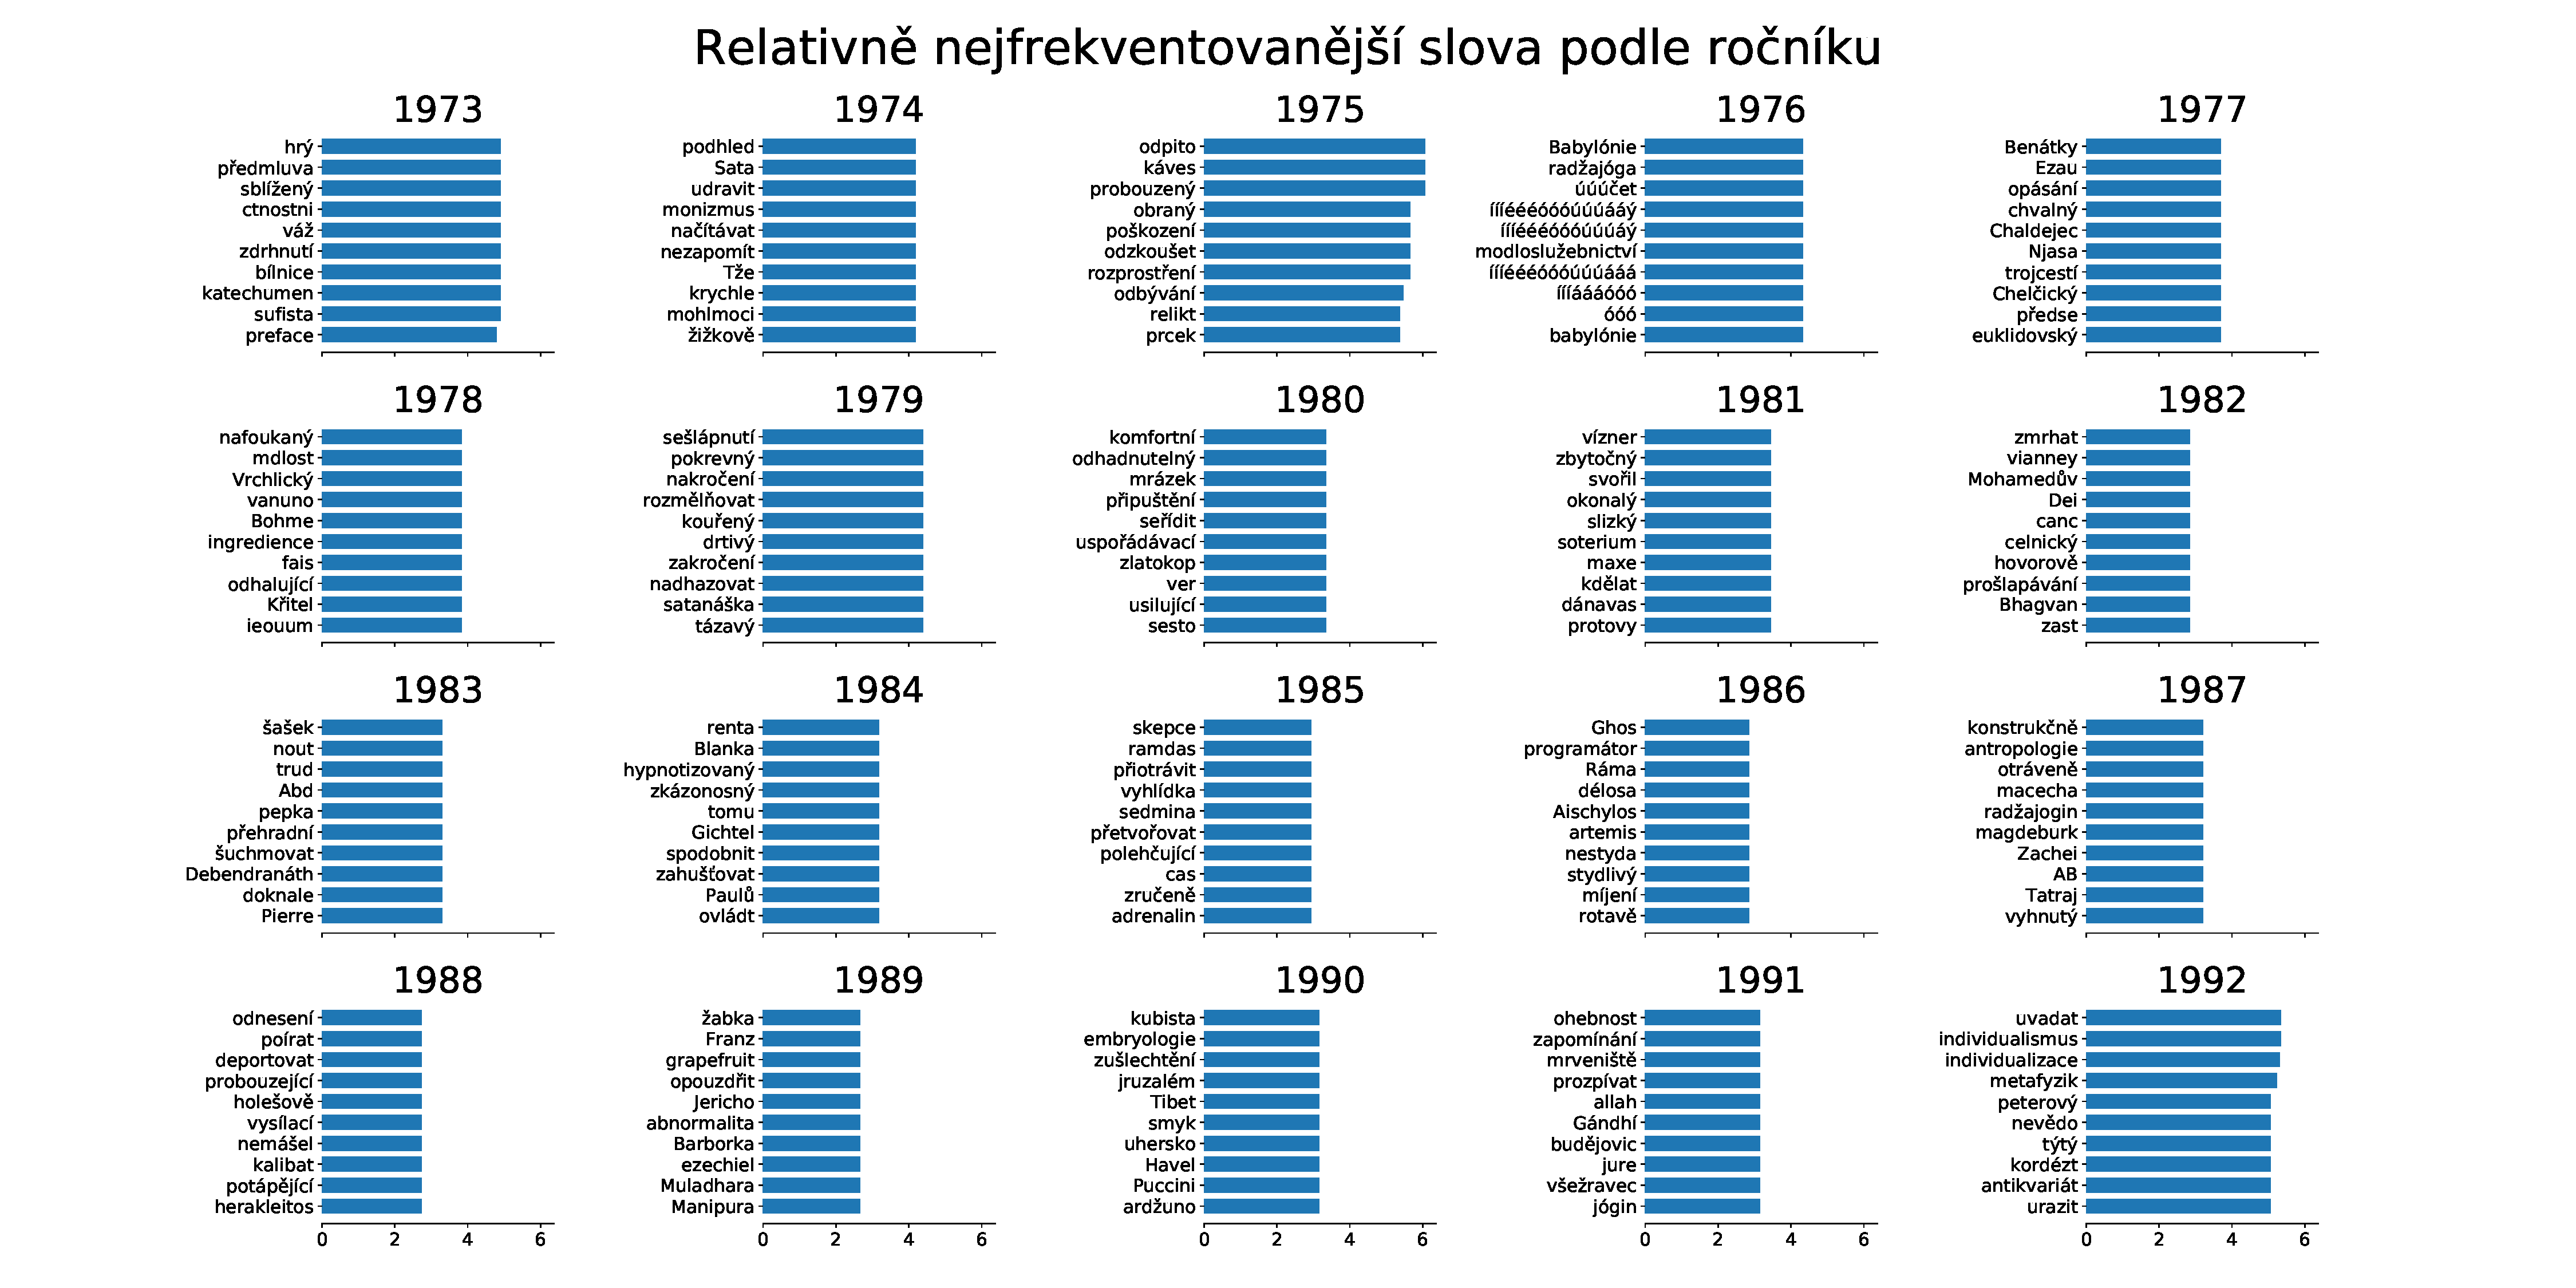
\includegraphics[scale=0.32, angle=90]{rc/topics-by-year-relfreq.pdf}
\caption{Slova s~nejvyšší relativní četností podle ročníku}
\label{fig:topic-by-year-relfreq}
\end{figure}

Naivní řešení je třeba konfrontovat s~řešením založeným za zavedených postupech.
V~oblasti extrakce klíčových slov z~textu je takovým zavedeným postupem
algoritmus \textit{TF-IDF}\cite{Beel2016-11Resea-32348}, anglická zkratka pro
,,term frequency -- inverse document frequency``, čili četnost pojmu -- inverzní
četnost dokumentů. Tento algoritmus upřednostňuje slova, která se vyskytují
často (term frequency) a upozaďuje slova, která se vyskytují často ve všech
dokumentech (inverse document frequency).

Adaptoval a použil jsem systém používající tf-idf jako váhu slov a
Kullbackovu-Leiblerovu divergenci jako míru pro porovnávání dokumentů.
Natrénoval jsem ho opět na celém korpusu Makoňových nahrávek a vyhodnotil pro
ročníky 1973 až 1992, opět po odfiltrování stop-slov a po lemmatizaci. Výsledek
je vidět na obrázku~\ref{fig:topic-by-year-kld}.

\begin{figure}[htpb]
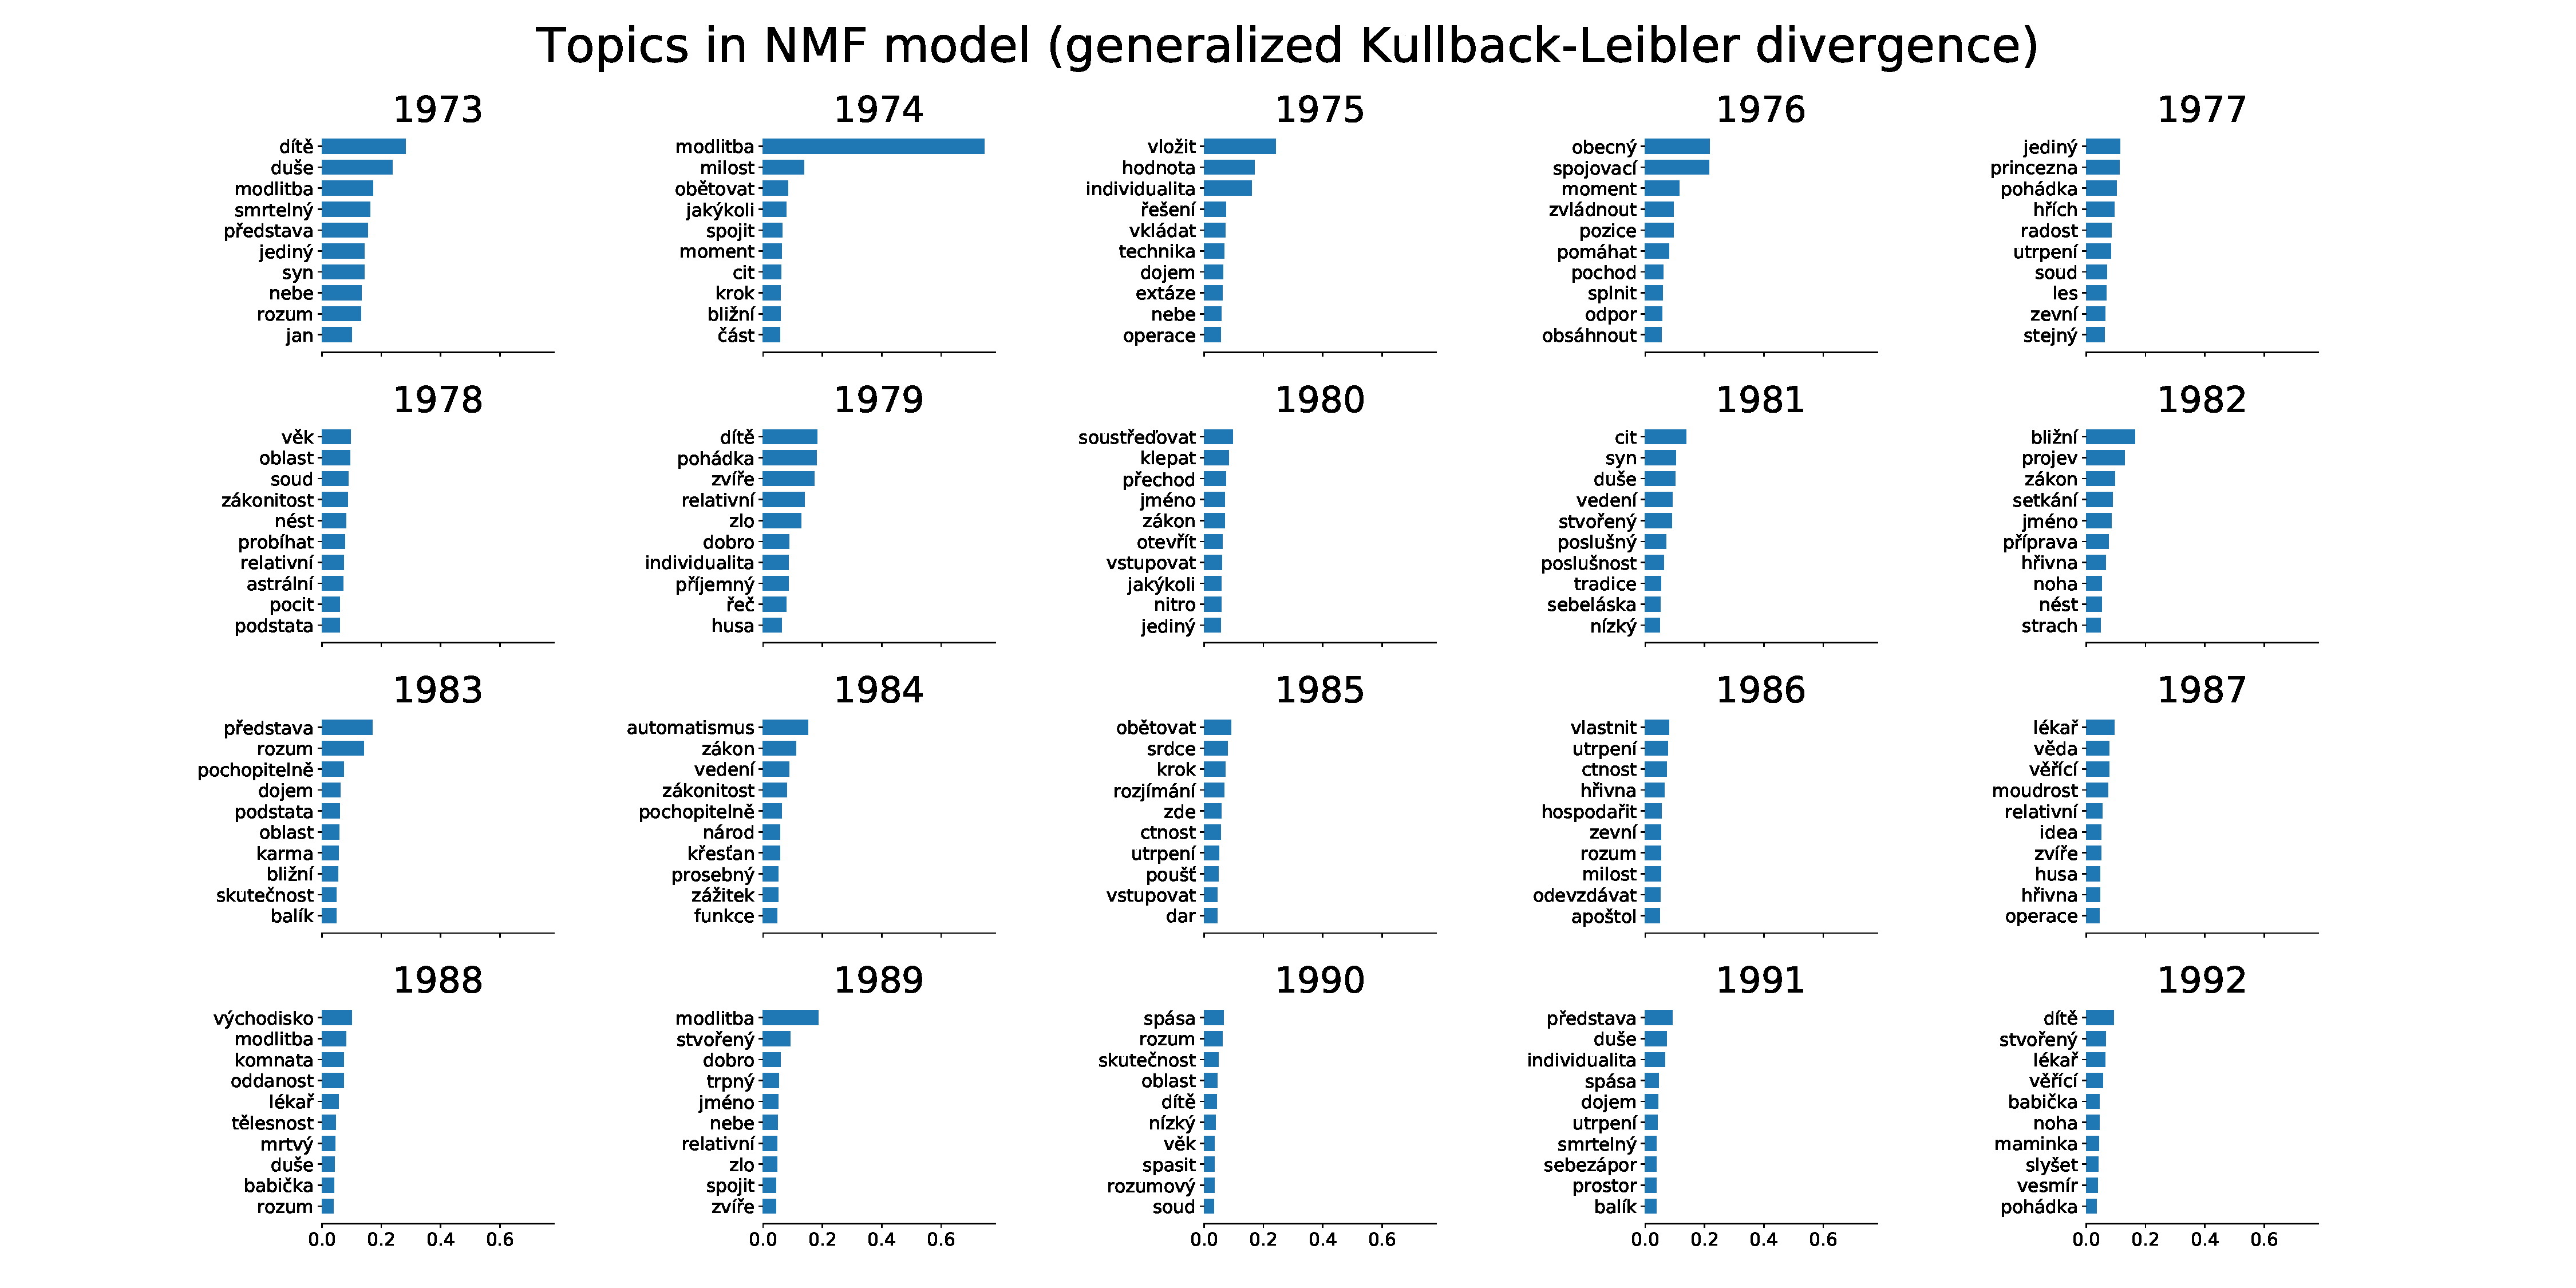
\includegraphics[scale=0.32, angle=90]{rc/topics-by-year-kld.pdf}
\caption{Slova s~nejvyšším skóre TF-IDF oproti Makoňovi podle ročníku}
\label{fig:topic-by-year-kld}
\end{figure}

Je pozoruhodné, že oba systémy nalezly zcela různá klíčová slova, přičemž obě
sady zcela zjevně odpovídají obashu Makoňových hovorů.

Oba výše představené systémy pracují na zálkladě porovnávání jednotlivých částí
Makoňova mluveného korpusu vůči celku. Odpovídají tedy na otázku, jaké téma se
diskutuje zde více než v~jiných pasážích. My se ale tážeme, o čem Makoň hovoří
vůbec. Tedy nás zajímají i témata, která se diskutují ve všech pasážích. Na to
musíme porovnat Makoňovy hovory s~jinými českými texty. Podle toho, jakou
referenční sadu textů bychom zvolili, bychom dostali odpovědi na různé otázky.
Pokud bychom například vzali za referenční sadu přepisy přednášek jiných českých
mystiků, dozvěděli bychom se, jaká slova používá Makoň víc než oni. Pokud bychom
si vzali jako referenční sadu současné české noviny, dozvěděli bychom se asi
hlavně, jak se Makoňův slovník liší od moderního českého žurnalistického
slovníku.

Vzhledem k~zaměření práce se spokojíme s~hotovým systémem
KER\footnote{http://lindat.mff.cuni.cz/services/ker/}, který také používá
algoritmus TF-IDF a jako referenční sadu používá texty z~české Wikipedie.
Pro každou jednotlivou nahrávku jsem nechal systém vyprodukovat klíčová slova --
byla zpravidla dvě -- a ve výsledcích jsem spočetl výskyty jednotlivých
nalezených slov.
Tabulka~\ref{tab:ker} ukazuje všechna nalezená slova, která se vyskytovala více
než jednou.

\begin{table}[htpb]
\begin{center}
\begin{tabular}{|r l|r l|r l|r l|}
\hline
\# & slovo & \# & slovo & \# & slovo & \# & slovo \\
\hline
575 & bůh	 & 8 & ráj	 & 4 & ctnost	 & 2 & syn	 \\
209 & člověk	 & 8 & otčenáš	 & 4 & činnost	 & 2 & svatební	 \\
106 & boží	 & 8 & babička	 & 4 & čaroděj	 & 2 & supramentální	 \\
96 & vůle	 & 7 & svatý	 & 4 & břemeno	 & 2 & stylizace	 \\
69 & modlitba	 & 7 & řeč	 & 3 & zlo	 & 2 & stupeň	 \\
42 & věčnost	 & 7 & prostředek	 & 3 & zážitek	 & 2 & starostlivost	 \\
35 & víra	 & 7 & pravda	 & 3 & zaujatost	 & 2 & sobectví	 \\
31 & vědomí	 & 7 & pokušení	 & 3 & zákon	 & 2 & smysl	 \\
30 & láska	 & 7 & karma	 & 3 & zainteresovanost & 2 & slepice	 \\
29 & úroveň	 & 7 & cit	 & 3 & vtělení	 & 2 & sebezlepšování	 \\
29 & správný	 & 6 & strach	 & 3 & vnitřní	 & 2 & sebepoznání	 \\
28 & poznání	 & 6 & smrtelný	 & 3 & trpný	 & 2 & samovolnost	 \\
24 & ježíš	 & 6 & podobenství	 & 3 & touha	 & 2 & samadhi	 \\
24 & duše	 & 6 & nitro	 & 3 & svět	 & 2 & ruysbroek	 \\
23 & bližní	 & 6 & formulace	 & 3 & spojovací	 & 2 & rozhodnutí	 \\
22 & život	 & 6 & dítě	 & 3 & spása	 & 2 & řešení	 \\
20 & představa	 & 6 & astrální	 & 3 & spánek	 & 2 & ramakrišna	 \\
17 & hřích	 & 5 & zákonitost	 & 3 & satan	 & 2 & prosebný	 \\
17 & duch	 & 5 & smrt	 & 3 & říma	 & 2 & prana	 \\
16 & učedník	 & 5 & pokora	 & 3 & relativní	 & 2 & poslušnost	 \\
16 & tělo	 & 5 & oddanost	 & 3 & radost	 & 2 & paměť	 \\
16 & stav	 & 5 & očistec	 & 3 & princezna	 & 2 & omyl	 \\
16 & pohádka	 & 5 & obraz	 & 3 & příjemný	 & 2 & očistný	 \\
16 & krista	 & 5 & duchovní	 & 3 & potopa	 & 2 & nebe	 \\
15 & stvořený	 & 5 & dobro	 & 3 & poklad	 & 2 & národ	 \\
15 & síla	 & 4 & zvíře	 & 3 & osvícení	 & 2 & muladharu	 \\
14 & rozum	 & 4 & zevní	 & 3 & okamžik	 & 2 & mrak	 \\
13 & východisko	 & 4 & vlastnost	 & 3 & noha	 & 2 & moudrost	 \\
13 & cesta	 & 4 & vitalita	 & 3 & milosrdenství	 & 2 & krok	 \\
12 & mysl	 & 4 & úkol	 & 3 & koncentrace	 & 2 & kristu	 \\
12 & kristus	 & 4 & událost	 & 3 & kelt	 & 2 & jho	 \\
11 & věc	 & 4 & tělesnost	 & 3 & jordánu	 & 2 & ííééóóúúáá	 \\
11 & milost	 & 4 & setkání	 & 3 & idea	 & 2 & hospodin	 \\
10 & zázrak	 & 4 & převtělování	 & 3 & eliáš	 & 2 & hospodář	 \\
10 & trpnost	 & 4 & moment	 & 3 & balík	 & 2 & drak	 \\
10 & individualita	 & 4 & maminka	 & 2 & zoufalství	 & 2 & dospělost	 \\
10 & hřivna	 & 4 & maličkost	 & 2 & zaujetí	 & 2 & chyba	 \\
10 & automatismus	 & 4 & lidský	 & 2 & vnuknutí	 & 2 & chrám	 \\
9 & utrpení	 & 4 & krize	 & 2 & vedení	 & 2 & bolest	 \\
9 & sebezápor	 & 4 & koncentrák	 & 2 & věda	 & 2 & anděl	 \\
8 & zjevení	 & 4 & klepání	 & 2 & ticho	 & 2 & analýza	 \\
8 & věčný	 & 4 & dojem	 & 2 & syntéza	 &   &                  \\
\hline
\end{tabular}
\caption{klíčová slova nalezená systémem KER}\label{tab:ker}
\end{center}
\end{table}

Je vidět, že hledáním klíčových slov můžeme dospět k~seznamu kandidátů na témata
v~množství více než hojném. Bohužel se zdá, že nelze než každého kandidáta
manuálně prověřit a zjistit, zda skutečně formuje téma, ke kterému se Makoň
soustavně vyjadřuje a u kterého by stálo za to posoudit jeho důležitost pro
Makoňovu nauku.

%utrpení:
%rovnováha mezi vnitřním a vnějším životem;
%nevědomost;
%nutnost odevzdání

%karma

%dobro a zlo

%zákonitost milosti Boží
